%----------------------------------------------------------------------------------------
%	INTRODUCTION
%----------------------------------------------------------------------------------------

\section{Einführung in die Thematik}

Innerhalb dieses in die Thematik einführenden Kapitels werden Grundlagen bezüglich der Bereiche, in denen sich das Projekt bewegt, aufgezeigt. Zunächst wird ein kurzer Überblick über die grundlegenden Prinzipien von HTTP und REST gegeben. Anschließend wird untersucht, wie APIs mithilfe von verschiedenen Deskriptionsformaten maschinenlesbar beschrieben werden können. Ziel dieser Untersuchung ist es, eine abstrakte Modellierung von REST APIs zu konzipieren, die verwendet werden kann, um eine API Spezifikation in eine interne Datenstruktur zu überführen, welche dann anschließend angereichert wird um automatisiert Artefakte wie Dokumentation und Test-Cases zu generieren. Im Zuge dessen wird im nächsten Kapitel analysiert, welche Möglichkeiten in diesem Feld bereits existieren.

\subsection{HTTP}

Das \emph{Hypertext Transfer Protocol} (HTTP) ist ein Anwendungsprotokoll zur Kommunikation über ein Netzwerk. HTTP ist das primäre Kommunikationsprotokoll im World Wide Web, und wurde von der Internet Engineering Task Force (IETF) und dem World Wide Web Consortium (W3C) in einer Reihe von RFC-Dokumenten (z.B. \href{https://tools.ietf.org/html/rfc7230}{RFC 7230}, \href{https://tools.ietf.org/html/rfc7231}{RFC 7231} und \href{https://tools.ietf.org/html/rfc7540}{RFC 7540}) standardisiert. In diesem Abschnitt werden die wichtigsten Charakteristiken aus den aufgeführten RFCs zusammengefasst. \\

Eine HTTP-Nachricht wird in der Regel über TCP übertragen, und besteht aus 4 Komponenten:

\begin{description}
	\item Verb / Methode: Operationstyp, der durchgeführt werden soll, beispielsweise das Anfragen einer Ressource.
    \item Ressourcenpfad: Ein Bezeichner, der angibt, auf welche Ressource die HTTP-Operation angewendet werden soll.
    \item Headers: Zusätzliche Metadaten, ausgedrückt als Liste von Key/Value-Paaren.
    \item Body: Enhält die Nutzdaten der Nachricht.
\end{description}

Das HTTP Protokoll erlaubt die folgenden Operationen bzw. Methoden:

\begin{description}
	\item \emph{GET}: Die angegebene Ressource soll im Body-Teil der Antwort zurückgegeben werden.
	\item \emph{HEAD}: Wie \emph{GET}, nur dass die Nutzdaten nicht zurückgegeben werden sollen. Dies ist nützlich, wenn nur überprüft wird, ob eine Ressource existiert, oder wenn nur die Header abgerufen werden sollen.
	\item \emph{POST}: Daten werden an den Server geschickt. Häufig wird diese Methode benutzt, um neue Ressourcen anzulegen.
	\item \emph{DELETE}: Die angegebene Ressource löschen.
	\item \emph{PUT}: Die angegebene Ressource mit neuen Daten ersetzen.
	\item \emph{PATCH}: Ändert eine Ressource, ohne diese vollständig zu ersetzen.
	\item \emph{TRACE}: Liefert die Anfrage so zurück, wie der Server sie empfangen hat.
	\item \emph{OPTIONS}: Liefert eine Liste der vom Server unterstützten Methoden auf einer Ressource.
	\item \emph{CONNECT}: Eine Tunneling-Verbindung über einen HTTP-Proxy herstellen, die normalerweise für verschlüsselte Kommunikationen benötigt wird.
\end{description}

Wenn ein Client eine HTTP-Anfrage sendet, schickt der Server eine HTTP-Antwort mit Headern und möglicherweise Nutzdaten im Body zurück. Darüber hinaus enthält die Antwort auch einen numerischen, dreistelligen Statuscode. Es gibt fünf Gruppen von Statuscodes, die durch die erste Ziffer identifiziert werden können:

\begin{description}
	\item \emph{1xx}: Wird für informierende Antworten verwendet, wie z.B. der Meldung, dass die Bearbeitung der Anfrage trotz der Rückmeldung noch andauert.
	\item \emph{2xx}: Wird zurückgegeben, wenn die Anfrage erfolgreich bearbeitet wurde. Der Server könnte beispielsweise weiter spezifizieren, dass eine neue Ressource angelegt wurde (201), z.B. durch einen POST-Befehl, oder dass im Antwortkörper nichts erwartet wird (204), z.B. durch einen DELETE-Befehl.
	\item \emph{3xx}: Wird für Umleitungen benutzt. So kann dem Client bspw. mitgeteilt werden, dass sich eine Ressource an einem neuen Ort befindet.
	\item \emph{4xx}: Bei der Bearbeitung der Anfrage ist ein Fehler aufgetreten, der durch den Client verursacht wurde. Dies können beispielsweise falsch formatierte Anfragen (400), Anfragen die vom Server nicht bearbeitet werden können (422), oder auch Anfragen auf nicht existierende Ressourcen (404) sein.
	\item \emph{5xx}: Bei der Bearbeitung der Anfrage ist ein Fehler aufgetreten, dessen Ursache beim Server liegt. 
\end{description}


\subsection{REST}

Representational State Transfer ist ein Muster von Ressourcenoperationen, das sich als Industriestandard für das Design von Webanwendungen etabliert hat \parencite[2]{battle2008bridging}. Während der traditionelle SOAP-basierte Ansatz für Web Services vollwertige Remote-Objekte mit Remote-Methodenaufruf und gekapselter Funktionalität verwendet, beschäftigt sich REST nur mit Datenstrukturen und der Übertragung ihres Zustands. \\

Representational State Transfer (REST) ist ein Softwarearchitekturstil, der die architektonischen Prinzipien, Eigenschaften und Einschränkungen für die Umsetzung von internetbasierten verteilten Systemen definiert \parencite[86]{fielding2000architectural}. REST basiert auf fünf Kernprinzipien \parencite[11]{tilkov2015rest}:

\begin{itemize}
	\item Ressourcen als Abstraktion von Informationen, identifiziert durch einen eindeutigen \emph{resource identifier} (die URI).
	\item Verknüpfungen / Hypermedia (HATEOAS). Jede Repräsentation einer Ressource sollte ebenfalls Links zu anderen relevanten Ressourcen enthalten. Da in der Praxis die Verwendung von HATEOAS jedoch recht selten ist \parencite[35--36]{rodriguez2016rest} werden im Folgenden auch solche APIs als RESTful bezeichnet, welche dieses Prinzip nicht umsetzen.
	\item Verwendung von Standardmethoden. Der Zugriff auf Ressourcen und deren Manipulation erfolgt mit den in HTTP definierten Standardmethoden. Jede Methode hat ihr eigenes standardisiertes Verhalten und erwartete Statuscodes.
	\item Unterschiedliche Repräsentationen. Clients kennen nicht direkt das interne Format und den Zustand der Ressourcen; sie arbeiten mit Ressourcendarstellungen (z.B. JSON oder XML), die den aktuellen oder beabsichtigten Zustand einer Ressource darstellen. Die Deklaration von Inhaltstypen in den Headern von HTTP-Nachrichten ermöglicht es Clients und Servern, Darstellungen korrekt zu verarbeiten \parencite[23]{rodriguez2016rest}.
	\item Statuslose Kommunikation. Interaktionen zwischen einem Client und einer API sind zustandslos, d.h. jede Anfrage enthält alle notwendigen Informationen, die von der API zur Verarbeitung benötigt werden müssen; es wird kein Zustand auf dem Server gespeichert.
\end{itemize}

\subsection{Spezifikationsformate}

In den letzten Jahren wurde viele Vorschläge gemacht, wie REST APIs menschen- und maschinenlesbar beschrieben werden können. Allen gemeinsam ist, dass die grundlegenden Eigenschaften von REST und HTTP (Ressourcen, Operationen, Requests, Responses, Parameter, usw.) in einem Modell zusammengefasst werden. Hierfür existieren eine Vielzahl von \emph{Description Languages} (DLs), von denen in diesem Abschnitt die wichtigsten betrachtet werden. Um zu identifizieren, welche DLs in der Industrie verwendet werden, kann auf die Ergebnisse der Untersuchung von \textcite{scherer2016description} zurückgegriffen werden. 

\begin{table}
\caption{API Description Languages, übersetzt aus \parencite[38]{scherer2016description}}
\label{tab:dls}
\scriptsize
\begin{tabularx}{\linewidth}{|p{2cm}|X|X|X|X|X|X|}
	\hline
    ~ & \textbf{API Blueprint} & \textbf{I/O Docs} & \textbf{Swagger} & \textbf{RAML} & \textbf{WADL} & \textbf{WSDL 2.0} \\
    \hline
    \textbf{Sponsor} & Apiary & Mashery & Reverb & MuleSoft & W3C & W3C \\
    \hline
    \textbf{Release} & April 2013 & Juli 2011 & Juli 2009 & Sep. 2013 & Aug. 2009 & Juni 2007 \\
    \hline
    \textbf{Format} & Markdown & JSON & JSON & YAML & XML & XML \\
    \hline
    \textbf{Google Ergebnisse ("[name]" + "REST")} & 27k & 4k & 860k & 86k & 88k & 14k \\
    \hline
    \textbf{StackOverflow Fragen (Titel)} & 49 & 2 & 1026 & 67 & 154 & 23 \\
    \hline
    \textbf{Github Projekte} & 269 & 34 & 1741 & 501 & 168 & - \\
    \hline
    \textbf{Github Spec Stars / Forks} & 2865/844 & 1646/408 & 2259/720 & 1962/123 & - & - \\
    \hline
\end{tabularx}
\end{table}

Aus Tabelle \ref{tab:dls} kann abgelesen werden, dass OpenAPI (ehemals Swagger) die populärste DL ist, wobei auch API Blueprint, RAML und WADL häufige Verwendung finden. WADL ist eines der frühesten Spezifikationsformate, welches allerdings aufgrund seiner Komplexität und begrenzten Unterstützung für die vollständige Beschreibung von REST-APIs in den letzten Jahren kaum noch benutzt wird \parencite[1]{ed2018automatic}. Dieser Abschnitt wird sich infolgedessen auf die Analyse von RAML, API Blueprint und OpenAPI beschränken. 

\subsubsection{Contract First und Contract Last}

Es kann im Wesentlichen zwischen zwei verschiedenen Ansätzen zur Definition des Vertrages, den eine API garantiert, unterschieden werden \parencite[272]{spichale2017api}:

\begin{itemize}
	\item \emph{Contract-First}. Bei diesem Ansatz wird zunächst der Vertrag (also die Spezifikation der API) geschrieben, und anschließend die Implementierung. Vorteilhaft ist hier der größere Fokus auf dem Design der Schnittstelle. In frühen Iterationen der Spezifikation kann in Abstimmung mit den Konsumenten der API mit geringen Aufwand der Vertrag gefestigt werden, sodass später bei der Implementierung weniger Änderungen anfallen. Nachteil ist, dass Entwickler mehr mit den eigentlichen Spezifikationen arbeiten müssen, und diese nicht automatisch generieren können.
	\item \emph{Contract-Last}. Bei diesem Ansatz existiert die Implementierung bereits, und die Beschreibung wird nachträglich erzeugt. Häufig können hier unterstützend Tools benutzt werden, welche die Spezifikation automatisch aus der Implementierung generieren, und der Entwickler muss meistens nur noch einige Annotationen anpassen. Da bei der automatischen Generierung Schemas in vielen Fällen dupliziert werden, kann dies zu mehr Aufwand führen, wenn manuelle Anpassungen vorgenommen werden müssen. Ebenso reduziert dies die Wiederverwendbarkeit von Spezifikationsteilen oder Schemas \parencite[1]{zhong2009contract}.
\end{itemize}

Bei beiden Ansätzen müssen Tests angelegt werden, die sicherstellen, dass die Implementierung nicht von der Beschreibung bzw. Dokumentation abweicht.

\subsubsection{JSON Schema}

Aufgrund seiner leichten Verständlichkeit für Menschen wie auch Maschinen hat sich JSON zum beliebtesten Format entwickelt, um API-Anfragen und Antworten über das HTTP-Protokoll zu senden \parencite[263]{pezoa2016foundations}. Durch diese Popularität ist allerdings auch der Bedarf gestiegen, mithilfe eines Schemas den Aufbau eines JSON Dokuments konkret zu definieren. Dies kann z.B. für die Validierung von Anfragen oder Antworten dienen. Ohne Integritätsschicht müssen viele Fälle berücksichtigt werden, die bei fehlerhaften API-Aufrufen auftreten, was vermieden werden kann, wenn eine Schemadefinition verwendet wird, um Dokumente herauszufiltern, die nicht die richtige Form haben. \\

JSON Schema ist eine einfache Schemasprache, die es Benutzern ermöglicht, die Struktur von JSON-Dokumenten einzuschränken. Die Definition ist noch lange kein Standard (die Spezifikation befindet sich derzeit im siebten Entwurf), aber es gibt bereits eine wachsende Anzahl von Anwendungen, die JSON-Schemadefinitionen unterstützen, und eine Vielzahl von Tools und Paketen, die die Validierung von Dokumenten anhand von JSON-Schema ermöglichen \parencite[264]{pezoa2016foundations}. \\

JSON Schema stellt mehrere Schlüsselwörter zur Beschreibung und Validierung von JSON Dokumenten zur Verfügung. Beispielsweise kann so der Typ von Daten festgelegt werden (\lstinline|null|, \lstinline|boolean|, \lstinline|object|, \lstinline|array|, \lstinline|number|, \lstinline|integer| oder \lstinline|string|). Es können ebenfalls vielzählige Restriktionen zur Validierung definiert werden, unter anderem: \lstinline|enum|, \lstinline|minimum|, \lstinline|maximum|, \lstinline|minLength|, \lstinline|maxLength|, \lstinline|regex| (Validierung anhand eines RegEx-Musters), \lstinline|required|, \lstinline|email|, \lstinline|date-time| und \lstinline|uri|.

\subsubsection{RAML}
RAML (\emph{RESTful API Modeling Language}) ist ein auf YAML basierendes Spezifikationsformat. Es wurde insbesondere für den \emph{Contract-First} Ansatz konzipiert, der Schwerpunkt liegt damit auf dem API-Design \parencites[277]{spichale2017api}[165]{tilkov2015rest}. Unterstützend dafür wurde von dem Unternehmen MuleSoft, einem der Autoren der Spezifikation, eine eigene IDE entwickelt, mit der REST APIs mithilfe von RAML designt, getestet und dokumentiert werden können (API Workbench). \\

Jedes RAML-Dokument beginnt mit der Angabe der RAML-Version und einigen allgemeinen Informationen zur API, wie Titel, URL und Version. Hier können ebenfalls Strukturierungshilfen wie Traits oder Datentypen definiert werden, welche dann im Rest des Dokumentes eingebunden und wiederverwendet werden können. Anschließend folgen die Beschreibungen der Ressourcen und Subressourcen. Zur Beschreibung von Requests und Responses können optional die bereits definierten Datentypen oder auch JSON-Schema Definitionen verwendet werden. Über \emph{Includes} kann die Spezifikation in mehrere Dateien aufgeteilt werden.

\begin{figure}[H]
  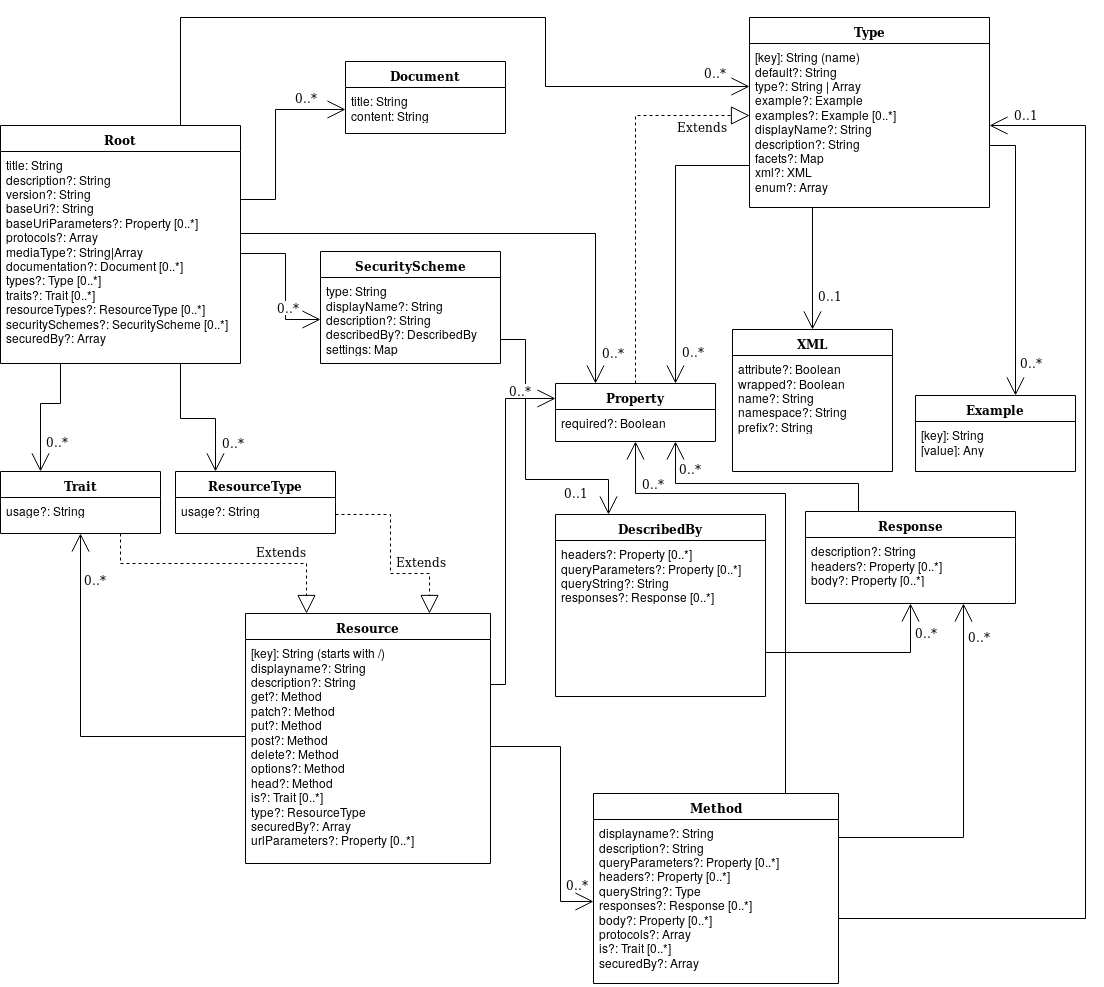
\includegraphics[width=\textwidth,height=\textheight,keepaspectratio]{../images/raml.png}
  \caption{Vereinfachtes RAML Metamodell}
  \label{fig:raml}
\end{figure}

\begin{figure}[H]
  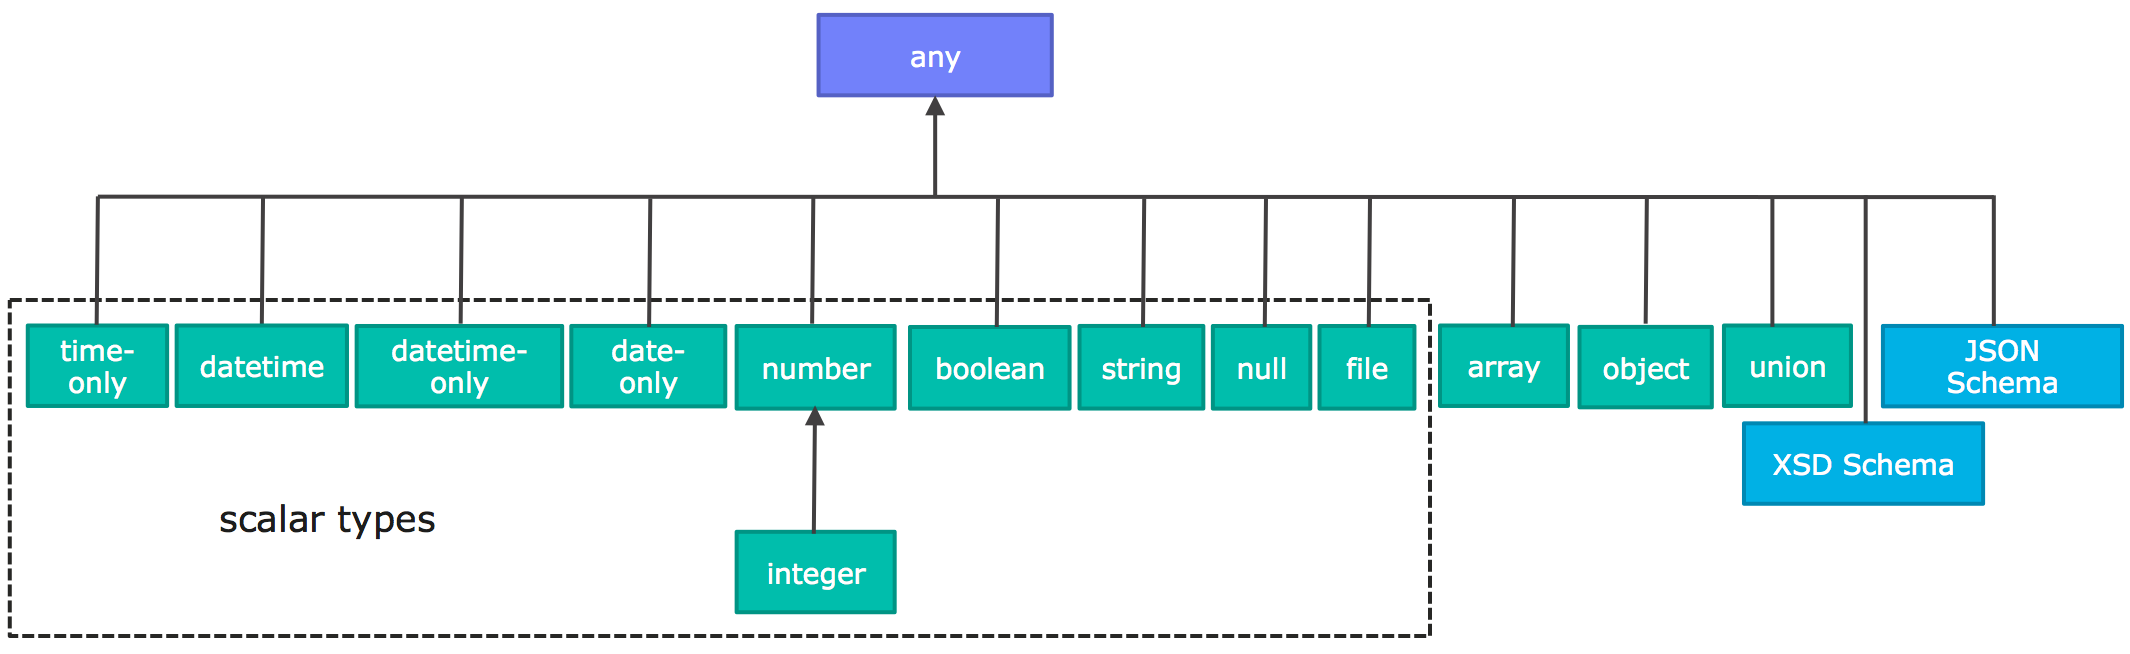
\includegraphics[width=\textwidth,height=\textheight,keepaspectratio]{../images/raml-data-types.png}
  \caption{RAML Datentypen (entnommen aus \cite{ramlspec})}
\end{figure}

Abhängig davon, welchen Datentyp eine Typdeklaration erweitert, können weitere Eigenschaften definiert werden. So kann ein Typ, welcher \lstinline|object| erweitert, noch Schlüssel wie \lstinline|properties| (Liste an \lstinline|Property| Objekten), \lstinline|minProperties| oder \lstinline|maxProperties| festlegen. Skalare Datentypen wie \lstinline|string| oder \lstinline|number| können ebenfalls zusätzliche Restriktionen ähnlich wie bei JSON Schema definieren (z.B. \lstinline|pattern|, \lstinline|minLength|, \lstinline|maxLength|, \lstinline|minimum| oder \lstinline|maximum|). Array-Typen können über \lstinline|items| (wiederum selber vom Typ \lstinline|Type|) festlegen, welchen Datentyp die einzelnen Elemente des Arrays haben. \\

In dem Diagramm (Abbildung \ref{fig:raml}) ausgelassen wurden Annotationen, ein Mechanismus mit dem in RAML fast jedem Objekt zusätzliche Metadaten hinzugefügt werden können. Dies wird häufig von Tools verwendet, um spezielle, für die Verarbeitung relevante Informationen zu definieren.

\subsubsection{API Blueprint}

API Blueprint ist eine Markdown-basierte Sprache, die von Apiary entwickelt wurde. Sowohl das Format als auch dessen Parser sind Open Source. Anders als bei OpenAPI und RAML wird bei API Blueprint mehr Wert auf Prosa gelegt, was durch die Verwendung von Markdown vereinfacht wird. Auf hohem Niveau ist die API Blueprint-Beschreibung für eine REST-API in der folgenden Struktur organisiert: \\

\begin{itemize}
	\item Metadaten: Enthält die API-Blueprint Version, den Namen der API und eine Beschreibung. Hier können ebenfalls zusätzliche Metadaten definiert werden, die dann von Tools benutzt werden können. Jedes API Blueprint Dokument startet mit dem \lstinline|FORMAT| Metadatum, welches die API Blueprint Version spezifiziert.
	\item Ressourcen und Ressourcengruppen: Enhalten die einzelnen Endpunkte, mit ihren Aktionen (bzw. Methoden), und den jeweiligen Requests und Responses.
	\item Datenstrukturen: Ähnlich wie Typen bei RAML können in API Blueprint eigene Datenstrukturen definiert werden, welche dann im Rest des Dokumentes wiederverwendet werden können. Die benutzte Syntax ist hierbei Markdown Syntax for Object Notation (MSON), eine ebenfalls von Apiary entwickelte, auf Markdown basierende  Alternative zu JSON Schema.
\end{itemize}

Das Dokument ist dabei in verschiedene Abschnitte aufgeteilt. Jeder Abschnitt, der durch ein Schlüsselwort definiert ist (z.B. einer URI Maske bei Ressourcen oder einem HTTP-Verb bei Aktionen), kann einen Identifikator, eine Abschnittsbeschreibung, sowie verschachtelte Abschnitte oder einen spezifisch formatierten Inhalt enthalten. 

\begin{figure}[H]
  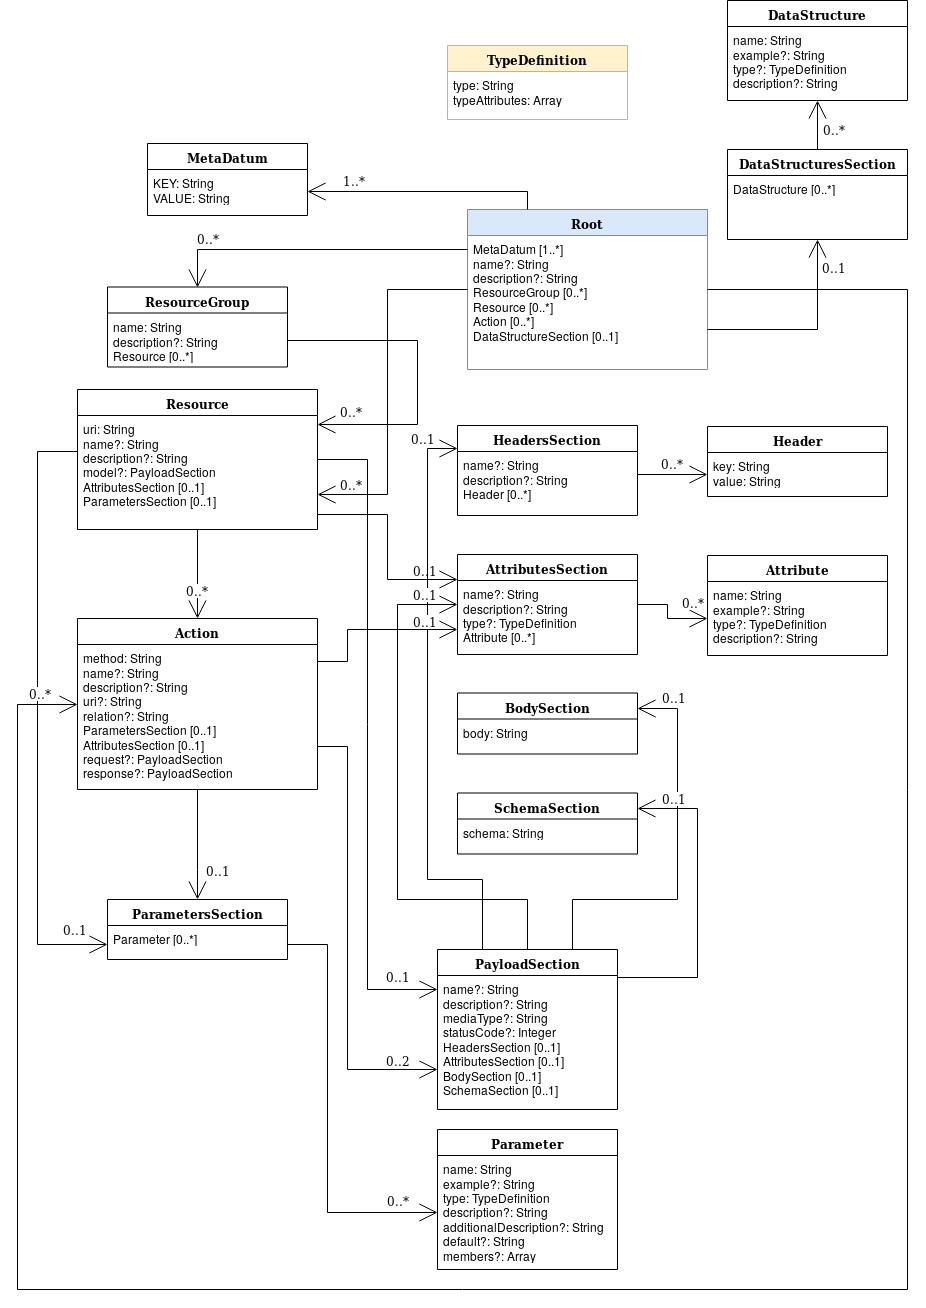
\includegraphics[width=\textwidth,height=\textheight,keepaspectratio]{../images/apib.png}
  \caption{Vereinfachtes API Blueprint Metamodell}
  \label{fig:apib}
\end{figure}

Das in Abbildung \ref{fig:apib} dargestellte Objekt \lstinline|TypeDefinition| ist eine Typdefinition nach MSON, bestehend aus einem Datentyp (\lstinline|string|, \lstinline|object|, \lstinline|array|, usw.) und mehreren optionalen Attributen (\lstinline|required|, \lstinline|optional|, \lstinline|fixed|, \lstinline|fixed-type|, \lstinline|nullable|, \lstinline|sample|, \lstinline|default|). Obwohl API Blueprint für die Definition von Datenstrukturen in der entsprechenden Sektion (\lstinline|DataStructuresSection|) lediglich MSON zulässt, kann in der Schemasektion ein JSON Schema eingebunden werden. Dieses kann aus einer externen Datei eingebunden werden, um somit die Wiederverwendbarkeit von Datenstrukturen zu simulieren. In der Body-Sektion kann ein JSON-Beispiel spezifiziert werden. \\

Auffallend ist, dass es in API Blueprint, anders als bei den anderen Spezifikationsformaten, keine Unterstützung für Authentifizierungsverfahren gibt. Diese können jedoch indirekt über die Header definiert werden. Ebenso fehlt die Unterstützung zur Versionierung der API. Externe Tools können hier jedoch mit speziellen Metadaten arbeiten.

\subsubsection{OpenAPI}

\subsubsection{Vergleich der Formate}

\subsection{Testing von REST APIs}
